%%%%%%%%%%%%%%%%%%%%%%%%%%%%%%%%%%%%%%%%%%%%%%%%%%%%%%%%%%%%%%%%%%%%%%%%%%%%%%%%%%%%%%%%%%%%%%%%%%%%%%%
%%%%%%%%%%%%%% Template Latex - Dissertação, Tese e Trabalho de Diplomação %%%%%%%%%%%%%%%%%%%%%%%%%%%
%% codificação UTF-8 - Abntex - Latex - 							     %%
%% Autor: Fábio Leandro Rodrigues Cordeiro  (fabioleandro@pucminas.br)                               %% 
%% Colaboradores: Prof. João Paulo Domingos Silva                                                    %%
%% Revisores normas NBR (Padrão PUC Minas): Helenice Rego Cunha e Prof. Theldo Cruz                  %%
%% Versão: 1.0     13 de Setembro 2013                                                               %%
%%%%%%%%%%%%%%%%%%%%%%%%%%%%%%%%%%%%%%%%%%%%%%%%%%%%%%%%%%%%%%%%%%%%%%%%%%%%%%%%%%%%%%%%%%%%%%%%%%%%%%%

\chapter{\uppercase{Introdução}}

A introdução deverá conter a natureza do trabalho, justificativa, objetivos, tema proposto e outros elementos para situar o trabalho.

A formatação deverá ter parágrafo recuado a 1,25 centímetros, fonte 12, espaçamento 1,5 justificado. Todo o texto deverá conter essa formatação com exceção para citações textuais, 
descritas adiante neste modelo. O título dos capítulos deve utilizar a formatação caixa alta, negrito, tamanho 12.

\section{\hspace{-0.3cm}Justificativa} %Esse hspace é por que as seções não ficam identadas quando n]ao colocado

Esta seção foi inserida para ilustrar uma seção terciária onde o título apresenta a seguinte configuração: caixa baixa, itálico, negrito, tamanho 12.

\chapter{\uppercase{Desenvolvimento}}

Todo título de seção ou subseção deverá ser seguido de texto.
Para as seções textuais utilizar numeração progressiva em algarismos arábicos, limitada até a seção quinária 
(NBR\sigla{NBR}{Norma Brasileira} 6024/2003) da ABNT\sigla{ABNT}{Associação Brasileira de Normas Técnicas}.
 Devem ser diferenciadas utilizando os recursos gráficos abaixo da mesma forma no sumário e no texto \cite{manualpuc}.

O título das seções primárias deve ser  Caixa alta, Negrito, tamanho 12.

\section{\hspace{-0.3cm}Seção secundária}

Os títulos das seções secundárias terão caixa baixa, negrito, tamanho 12.

\subsection{\hspace{-0.3cm}Seção terciária}

Caixa baixa, itálico, negrito, tamanho 12.

\subsubsection{\hspace{-0.3cm}Seção quartenária}
 
 Caixa baixa, sublinhado, negrito, tamanho 12.
 
\vspace{0.5cm} 
 \noindent{2.1.1.1 Seção quinária} % \paragraph{\hspace{-0.3cm}Seção quinária} 
\vspace{0.5cm}

 Caixa baixa, sem negrito, tamanho 12.

  
 \chapter{\uppercase{Elementos flutuantes}}


Elementos inseridos no texto como imagens, tabelas, algoritmos etc.


\section{\hspace{-0.3cm}Inserções de ilustrações}

As ilustrações devem ser inseridas seguindo o exemplo abaixo da Figura \ref{fig:figura1}. 

% Figura
\begin{figure}[ht]
	\centering	
	\caption[\hspace{0.1cm}Grade Computacional.]{Uma Grade Computacional como fonte transparente}
	\vspace{-0.2cm}
	\includegraphics[width=.6\textwidth]{figuras/grade-comp.png}
	% Caption centralizada
% 	\captionsetup{justification=centering}
	% Caption e fonte
	 \vspace{-0.2cm}
	\\\textbf{\footnotesize Fonte: \cite{cap-livro} }
	\label{fig:figura1}
\end{figure}

Recomenda-se a colocação das ilustrações de forma centralizada, dentro das margens. 
Caso não seja possível, devem-se utilizar recursos como: a) utilizar letras tamanho menor ao padrão do texto; b) imprimir a
ilustração no sentido vertical; c) imprimir em folha A3 ou superior e
dobrá-la até atingir o tamanho da folha A4 \cite{manualpuc}. 

% Figura
\begin{center}
	\centering	
 	\textbf{Exemplo de um gráfico} \\
%  	  \vspace{0.cm}
	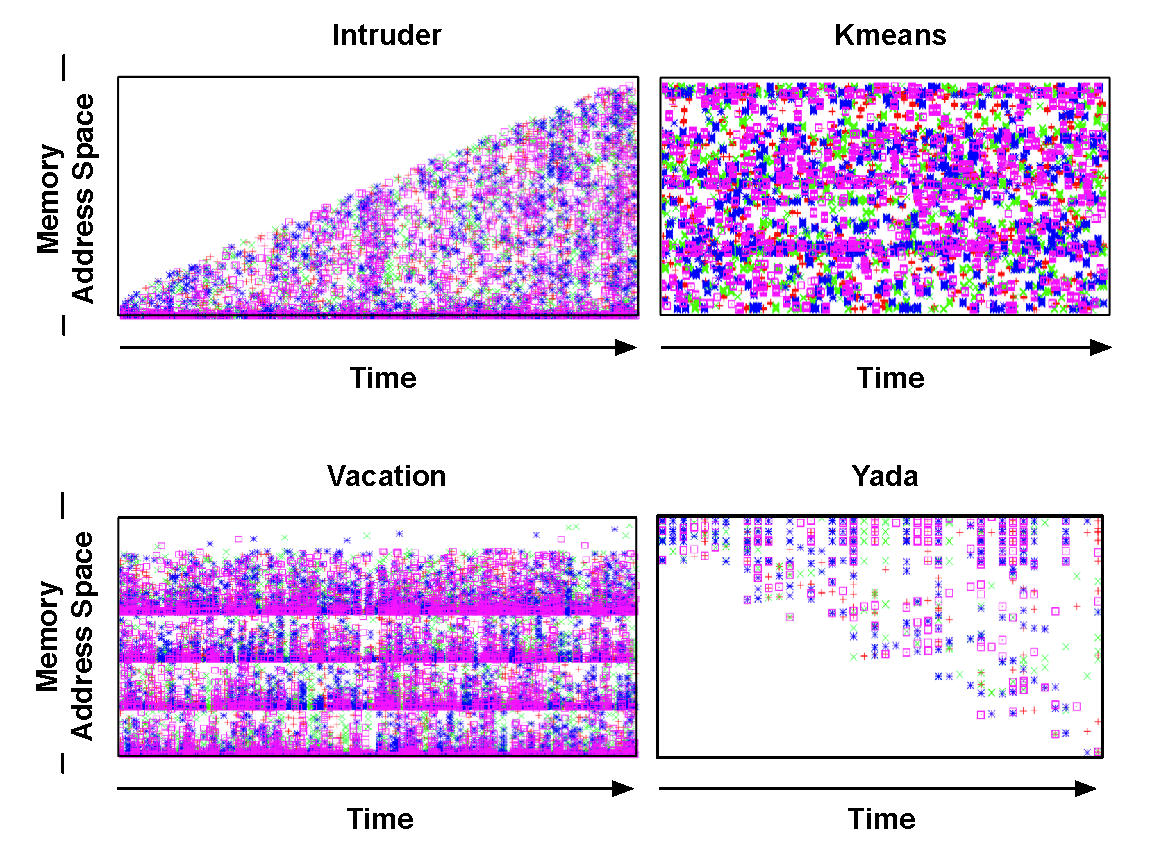
\includegraphics[width=.7\textwidth]{figuras/graficos/access_patterns.eps}
	% Caption centralizada
% 	\captionsetup{justification=centering}
	% Caption e fonte
	 \vspace{-0.3cm}
	\\\textbf{\footnotesize Fonte: \cite{tese}}
	\label{fig:grafico1}
\end{center}

Para gráficos, quadros e tabelas, cujos dados foram extraídos da própria pesquisa, 
usar a expressão: Dados da pesquisa. Veja o exemplo no Quadro \ref{quadro1}.

% Figura
\begin{figure}[ht]
	\centering	
	\caption[\hspace{0.1cm}Exemplo de tela de software.]{Exemplo de tela de software}
	  \vspace{-0.2cm}
	\includegraphics[width=.9\textwidth]{figuras/tela1.png}
	% Caption centralizada
% 	\captionsetup{justification=centering}
	% Caption e fonte
	 \vspace{-0.1cm}
	\\\textbf{\footnotesize Fonte: \cite{tela1}}
	\label{fig:tela1}
\end{figure}

% \section{\hspace{-0.3cm}Tabelas}

As tabelas são fechadas nas laterais. Entre os elementos da tabela devem haver linhas. Um exemplo é a tabela \ref{tab:tabela1}. 

% Tabela
\begin{table}[htb]
	\centering
	\caption{\hspace{0.1cm} Exemplo de uma tabela}
	\vspace{-0.3cm} % espaço entre titulo e tabela
	\label{tab:tabela1}
	% Conteúdo da tabela
	\begin{tabular}{l|c|c}
  \hline
    \textbf{Imagem}	& \textbf{transferência} & \textbf{tempo} \\
    \hline
     estação 1	& 7,72 MB/s &  1:22:18 \\
     estação 2	& 7,72 MB/s &  1:22:17 \\
     estação 3	& 7,59 MB/s & 1:24:25 \\
     estação 4  & 7,53 MB/s & 1:43:27 \\
     estação 5	& 6,14 MB/s  &  1:24:41 \\
     estação 6  &  7,50 MB/s & 1:23:53 \\
     estação 7  & 7,58 MB/s  &  1:24:02 \\
     estação 8  & 7,8 MB/s  &  1:29:06 \\
     estação 9  & 7,9 MB/s  &  1:30:05 \\
     estação 10 & 8,0 MB/s  &  1:32:03 \\
     \hline
 \end{tabular}
 	\vspace{.1cm}  %espaço entre tabela e fonte
	\small
	% Fonte
	{\footnotesize\\ \textbf{Fonte: \cite{monog-fabio}}}
\end{table}

\section{\hspace{-0.3cm}Quadros}

Os quadros diferem das tabelas por apresentarem dados textuais.
Esses dados podem ser esquemáticos, comparativos ou descritivos.

\vspace{0.7cm}

   \begin{center}
          \centering
       	\textbf{Quadro 1 - Bandas de Rock}\\
% 	\vspace{-0.3cm} % espaço entre titulo e tabela
        \label{quadro1}
	\begin{tabular}{|c|c|c|c|} \hline
	\multicolumn{4}{|c|}{Bandas de Rock} 	  \\ 
		\hline 	Progressivo & Pink Floyd & Yes	& Yesterday \\ 
		 \hline Metal  & Metallica & Iron Maidam & Black Sabath \\ 
		\hline 	Classic & Led Zeppelin	& The Doors & Beatles \\ 
		\hline 	Punk & Ramones & Black Flag & NOFX	\\ 
		\hline 	Nacional & Ira & Engenheiros & Vinil	\\ 
		\hline
	\end{tabular}
	\vspace{0.1cm} 
	{\footnotesize\\ \textbf{Fonte: Dados da pesquisa}}
   \end{center}


\section{\hspace{-0.3cm}Inserção de algoritmos}

Para inserir um algoritmo, utilizar o exemplo do algoritmo da Figura \ref{alg:rnagenerica}.
Todos os algoritmos devem ser inseridos como figura, indicada por nome e  fonte. Caso 
forem de própria autoria, isso deverá ser mencionado na fonte, como elaboração feita pelos autores.

% algoritmo
% \begin{figure}[ht]
\begin{center}	
	% Arquivo da figura
% 	\caption[\hspace{0.1cm} Texto da figuras.]{Algorítmo CAC RD Neural}
        \textbf{Algoritmo CAC RD Neural}
	\vspace{-0.3cm}
\begin{minipage}[ht]{13cm}
\begin{algorithm}[H]
  \footnotesize
  \caption{CAC-RD Neural}
  \label{alg:rnagenerica}
  \begin{algorithmic}[1]
      \STATE \textbf{Entrada:} Requisição da chamada
    \STATE \textbf{Saída:} Aceitação ou bloqueio da solicitação
    
    \STATE Preenche o vetor de $attributes.size+1$ atributos com os valores dos atributos, sendo a primeira posição do vetor preenchida com o valor 1
		\STATE $hidden\_layer\_size =  attributes.size*2+1;$

    \FOR{$i$ = 1 to $attributes.size+1$}
    	\STATE \textbf{normalizar}($Entrada_i$)
    \ENDFOR

		\STATE $double [] net = new double [hidden\_layer\_size];$
    \STATE $net = hidden\_layer\_weights * attributes;$
   	\FOR{$i$ = 0 to hidden\_layer\_size}
			\STATE $net [i] = 1.0 / (1.0 + exp((-1.0)*net[i]));$
		\ENDFOR

		\STATE $double [] ipVector = new double [hidden\_layer\_size+1];$
    \STATE $ipVector [0] = 1.0;$
   	\FOR{$i$ = 1 to $hidden\_layer\_size+1$}
			\STATE $ipVector [i] = net [i-1];$
		\ENDFOR
		
		\STATE $output = output\_layer\_weights *  ipVector;$
    \STATE output = \textbf{desnormalizar}(Saída)
    \STATE \textbf{net\_update} (requisition);
    
    \STATE \textbf{Retorna} output; FIM
  \end{algorithmic}
\end{algorithm}
% \vspace{-0.3cm} % espaço entre algoritmo e fonte

\small \centering \textbf{\footnotesize Fonte: \cite{mestrado}.}
\end{minipage}
\end{center}
% \end{figure}

Para ilustrações criadas ou adaptadas a partir de outras ilustrações, usar as expressões: 
“Adaptado de...” ou “Criado pelo autor`` com dados extraídos de...
   
   
\chapter{\uppercase{Citações}}


Referências deverão ser adicionadas no arquivo \textit{bibliografia.bib}. Cada referência deverá ser adicionada conforme o padrão de normalização da PUC, 
o qual poderá ser obtido na página da biblioteca da PUC Minas \cite{manualpuc}. 

Todas as publicações citadas no texto deverão ter correspondente nas referências, e as indicações de autoria da citação e do ano deverão ser idênticas aos dados da referência.


\section{\hspace{-0.3cm}Citação livre ou indireta}

Quando se reproduzir ideias, sem transcrever as palavras do autor, a indicação da página é opcional.

Exemplos desse tipo de citação:
\begin{enumerate} 
 \item [a)] Citação com um autor \cite{knuth}. 
 \item [b)] Citação de artigos em revistas com dois autores \cite{artigo01}.
%  \item [c)] Trabalho em congresso com três autores \cite{dovzan:01}.
 \item [d)] Trabalhos com mais de três autores \cite{congresso}.
\end{enumerate}

\section{\hspace{-0.3cm}Citação direta ou textual}

Transcrição literal de textos de outros autores. Nesse caso, deverão ser especificadas as páginas consultadas. 
Se desejar, poderão ser grafadas em itálico para melhor visualização.

\subsection{\hspace{-0.3cm}Textual Curtas}

Quando curtas (até 3 linhas) serão inseridas na sequência normal do texto, entre aspas com as mesma formatação.

\subsection{\hspace{-0.3cm}Textual Longas}

Citações longas (mais de 3 linhas) deverão constituir um parágrafo independente, recuado a 4 cm da margem esquerda, 
com letra tamanho 10 e digitado em espaço simples, sem aspas.
\begin{citacaodireta}
Hegel chama trabalho à forma específica da satisfação das necessidades, que
distingue da natureza o espírito existente. Assim como a linguagem infringe
a imposição da intuição e ordena o caos das múltiplas sensações em coisas
identificáveis, assim o trabalho infringe a imposição do \hspace{0.1cm}desejo \hspace{0.1cm}imediato \hspace{0.1cm}e
suspende, por assim dizer, o processo de satisfação das necessidades.
\cite[25]{habermas}.
\end{citacaodireta}


% Artigo \cite{whatershed:01}

\subsection{\hspace{-0.3cm}Textual de outros idiomas (Tradução)}

\begin{citacaodireta} 
Um \textit{cluster} é um computador paralelo construído de componentes e processos de \textit{software} (tal como sistema de \textit{software}). 
Um \textit{cluster} é formado de nós, cada um contendo um ou mais processadores, memória que é compartilhada por todos os processadores do nodo 
(somente eles), e dispositivos periféricos adicionais (tais como discos), conectados pela rede e que permitem tráfego de dados entre os nós...
\cite[p. 10, tradução nossa]{groupp}\footnote {  … a cluster is a parallel computer that is constructed of commodity  componets and runs 
(as its system software) commodity software. A cluster is made of nodes, each conteining one or more processors, memory that is  shared 
by all of the processors in (and only on) the node, and addtional peripheral devices (surch as disks),
 connected by network that allows data to move between the nodes}.

\end{citacaodireta}
 
\section{\hspace{-0.3cm}Exemplos de citações} 

Alguns exemples de citações mais utilizadas e/ou que geram algumas dúvidas. É válido observar que não citaremos
todas as possibilidade de citações da norma da PUC Minas, sendo assim é de extrema relevância que se consulte 
o documento no site da Biblioteca da PUC Minas para maiores esclarecimentos acerca de citações. O manual pode
ser visto em \citeonline{manualpuc}.

\subsection{\hspace{-0.3cm}Citação de monografia, dissertação e tese}

Exemplo de citação de monografia de conclusão de curso de graduaçã ou especialização pode ser vista em \citeonline{monog-fabio}.

Exemplo de dissertação de mestrado é referida como \citeonline{mestrado}.

E para o caso de doutorado é citado da seguinte forma, Góes (\citeyear{tese}). Neste exemplo é válido observar a forma
como esta sendo escrito no documento \LaTeX, pois citações que compreendem no texto o nome do autor como sua parte, necessitam 
do parâmetro \verb$\citeonline{}$. Porém existe um problema com palavras acentuadas não permitindo o uso do comando em sua forma normal.

\subsection{\hspace{-0.3cm}Livros e partes de livros}

Exemplo de capítulo de livro ficam conforme este exemplo \cite{cap-livro}.

Livros conforme anteriormente citados, e agora na sua forma de citação no corpo do texto e com duas citações juntas, veja os exemplos \citeonline{knuth,groupp}.
Caso esta citação não fizesse parte do texto seria referencia desta forma \cite{knuth,groupp}.

Citações institucionais ou documentos técnicos de alguma entidade devem ser citados desta forma, \cite{pmbok}

\subsection{\hspace{-0.3cm}Tela de software}

Para  citar a tela de um \textit{Software} faça da seguinte forma, \citeonline{tela1}.

\subsection{\hspace{-0.3cm}Citações da Biblia Sagrada}

A Bíblia está dividida em duas grandes partes: O Antigo Referências: Testamento e o Novo Testamento, que são divididos em livros, capítulos e versículos. 
Portanto, a citação de partes da Bíblia deve apresentar o título do livro de forma abreviada ou por extenso, o número do capítulo e o número do versículo.


\begin{citacaodireta}

% Moisés estendeu a mão sobre o mar. Com um forte \hspace{-0.1cm} vento \hspace{0.1cm} leste a \hspace{0.1cm}sobrar a
noite toda, o Senhor repeliu o mar e o pôs a seco. As águas se fenderam e
os filhos de Israel entraram no meio do mar a pé enxuto, enquanto as águas
formavam uma muralha à direita e à esquerda deles (\citeauthor{biblia}14,21).

\end{citacaodireta}

\chapter{\uppercase{Conclusão}}

Discussão dos resultados obtidos na pesquisa, onde se verificam as observações pessoais 
do autor. Poderá também apresentar sugestões de novas linhas de estudo.

A conclusão deve estar de acordo com os objetivos do trabalho.

A conclusão não deve apresentar citações ou interpretações de outros autores.

\section{\hspace{-0.3cm}Trabalhos futuros}

Sugestões de estudos posteriores são ser adicionados subseção deste capítulo de conclusão.
